\subsection*{Introduction}

\subsubsection*{---Problem Definition} \par
The main goal of this project is to demonstrate the viability of a variable impedance controller with the use of a one-dimensional prototype. Variable impedance control utilizes user input in order to achieve a desired state of mobility. The system senses a force and responds by changing its impedance to match the desired input parameters of the user. The user will be able to control the virtual weight, damping, and spring force. These virtual parameters will dictate how the system performs while being used. \par
There are many applications for this research and while only a simple prototype, the implications are far-reaching. With variable impedance control, a heavy object can feel lighter and be easier to maneuver. Lighter objects that don't provide enough feedback for a human can have their apparent weight increased. When human control and reasoning is desired over robot logic, variable impedance control can make a difference. This report details the design and construction of a one-dimensional cart prototype that successfully demonstrates the capability of a variable impedance controller.\par

\subsubsection*{---Functional Requirements} \par
<<<<<<< HEAD
At the beginning of the design phase, we set target values for the settling time and percent overshoot, found in \ref{specs}.
\begin{table}[H]
	\centering
	\caption{Functional Specifications}
	\label{specs}
	\begin{tabular}{|l|l|}
		\hline
		Target Requirement &          \\ \hline
		\%OS               & 5\%      \\ \hline
		Settling Time      & 0.15 sec \\ \hline
	\end{tabular}
\end{table}
 Using the targets, an appropriate motor and amplifier were attained. In selecting a motor, a reference had to be used to run simulations, so a motor with a torque constant of .11 N/m was used in tandem with an amplifier with a gain of .79 A/V. Using these sample motor and amplifier constants in the model, simulations were run through Simulink to verify that such a motor and amplifier combination would suffice by checking the maximum current, voltage, torque and rpm required against what the motor and amp could supply. Cases with low mass and damping proved to have the highest torque and current requirements because the velocity profile of such a system would involve very high accelerations. From the results we decided that damping must always be included in the reference system to limit the necessary torque. \par
After the design was finalized a functional specification map was created to guide the user's inputs. The motivation for this was observing that the low mass, low damping case performed reasonably well as long as the force input was small. In addition, a greater force could be applied if either the damping or mass was increased. This led to the conclusion that the limitations on the reference system parameters were actually coupled. Considering the restrictions that either increasing the mass or the damping would put on the acceleration of the reference system for a given force input, this conclusion seemed logical. To create the mapping, a calculation was done on the transfer function relating the force input to the required motor current.\begin{equation}
=======
At the beginning of the design phase, target functional specifications were set. The specifications were based on ambitious but attainable goals for percent overshoot and settling time. Using the targets, the motor and amplifier were sized. In selecting a motor, a reference had to be used to run simulations, so a motor with torque constant of .11 N/m was used in tandem with an amplifier with a gain of .79 A/V. Using these sample motor and amplifier constants in the model, simulations were run through Simulink to verify that such a motor amplifier combination would suffice by checking the maximum current, voltage, torque and rpm required against what the motor and amp could supply. Cases with low mass and damping proved to have the highest torque and current requirements because the velocity profile of such a system would involve very high accelerations. From the results it was decided that damping must always be included in the reference system to limit the necessary torque.
\begin{figure*}[th!]
	\centering
	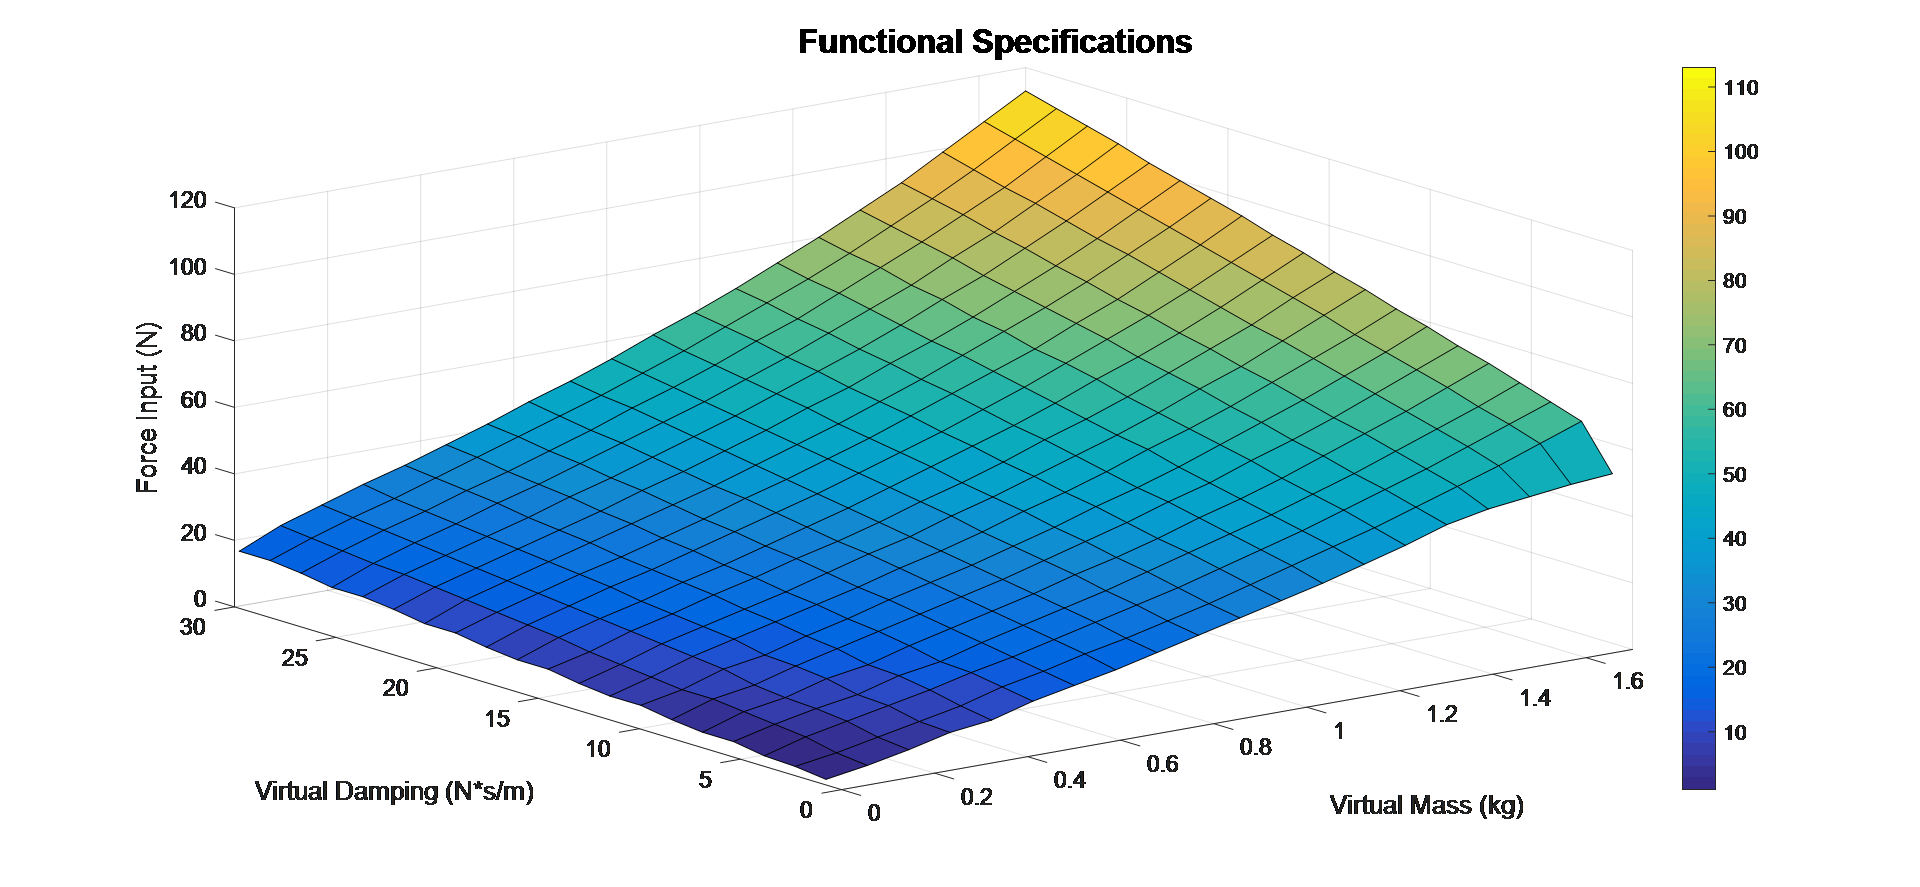
\includegraphics[width=1\linewidth]{Images/Functional_Specifications_Mapping}
	\caption{3D mapping of the maximum human input force for varying virtual mass and damping. Virtual stiffness is set to 5 N/m}
	\label{fig:Functional_Specifications_Mapping}
\end{figure*}
\newline \indent After the design was finalized a functional specification mapping was developed to guide the user's inputs. The motivation for this was observing that the low mass, low damping case performed reasonably well as long as the force input was small. In addition, a greater force could be applied if either the damping or mass was increased. This led to the conclusion that the limitations on the reference system parameters were actually coupled. Considering the restrictions that either increasing the mass or the damping would put on the acceleration of the reference system for a given force input, this conclusion seemed logical. To create the mapping, the transfer function relating the force input to the required motor current was calculated.\begin{equation}
>>>>>>> master
I = \frac{[K_{P}s+K_{I}][(\epsilon-M)s^{2}-Bs-K]}{[\frac{\epsilon}{K_{A}}s^{2}+\frac{K_{P}K_{M}}{r}s+\frac{K_{I}K_{M}N}{r}][Ms^{2}+Bs+K]}F
\end{equation}
Where 
\begin{equation}
\epsilon = M+\frac{JN^{2}}{r^{2}}
\end{equation}
\newline \indent The transfer function depends on the parameters of both the reference and actual systems, as predicted, but not in any clearly identifiable way. The mapping was generated numerically using successive approximation to determine what applied force would result in the current requirement exceeding the limitations of the amplifier, about 4.8 A. The parameters varied were the mass and damping, as the relationship between the spring and acceleration was less complex and more intuitive and the input force was a critical component of any mapping.
\newline \indent The mapping shown in Figure 1 is just a small portion of the effective range. This portion was selected because it demonstrates the very small force that can be applied when the reference system has very low mass. The maximum value of force shown is near 111 N which is approximately the limit of the load cell range. Theoretically, the force possible to apply would continue to increase beyond this point but the load cell would not read it as a greater force, so the system cannot handle greater forces regardless. If the load cell range was not the limiting factor, it is presumed that the force would increase with the damping and mass until the torque required to prevent the acceleration of the real system going beyond the reference system's response for the input force. In this way, the lower range of the the functional specification mapping can be seen as dependent on the ability of the motor to increase the acceleration of the real system and the higher range of the functional specification mapping can be seen as dependent on the ability of the motor to decrease the acceleration of the real system.
